\appendix

\clearpage{\renewcommand{\appendixname}{Anexos}}
\addappheadtotoc


\begin{comment}
	

\renewcommand\thefigure{.\arabic{figure}}  
\setcounter{figure}{0} 
\renewcommand\figurename{\footnotesize FIGURA A \hspace{-1.6mm}}
\def\figureautorefname{Figura A \hspace{-2mm}}

\end{comment}

\chapter{Elementos para la configuración del componente \textit{AutoML Clasificación (pre-procesado)}}\label{aped:1}
%\addcontentsline{toc}{section}{Anexo I: Elementos para la configuración del componente para la \textit{HPO}}

\begin{figure}[H]
	\centering
	\includegraphics[width=\textwidth]{"figuras/anexos/2.2 Configuracion modelo-----Configuración del componente AutoML Clasificación (Optimización de Hiperparámetros)"}
	\caption{Flujo KNIME para la configuración del componente \textit{AutoML Clasificación (pre-procesado)}}
	\label{anex:config-hpo-comp}
\end{figure}

\chapter{Evaluar la columna objetivo en el componente\textit{ AutoML Clasificación (Optimización de Hiperparámetros)}}\label{aped:2}
%\addcontentsline{toc}{section}{Anexo II: Elementos para la evaluación de la columna objetivo del componente para la \textit{HPO}}

\begin{figure}[H]
	\centering
	\includegraphics[width=\textwidth]{"figuras/anexos/2.2.2 Evaluar columna objetivo"}
	\caption{Flujo KNIME para la evaluación de la columna objetivo en el componente\textit{ AutoML Clasificación (Optimización de Hiperparámetros)}}
	\label{anex:evaluar-columna-obj}
\end{figure}
	

\chapter{Graficar columna objetivo binaria para el componente \textit{ AutoML Clasificación (Optimización de Hiperparámetros)}}\label{aped:3}
%\addcontentsline{toc}{section}{Anexo III: Elementos para graficar la columna objetivo binaria del componente para la \textit{HPO}}

\begin{figure}[H]
	\centering
	\includegraphics[width=\textwidth]{"figuras/anexos/2.2.2 Graficar Clase binaria"}
	\caption{Flujo KNIME para graficar cuando la columna objetivo es binaria en el componente\textit{ AutoML Clasificación (Optimización de Hiperparámetros)}}
	\label{anex:grafic-binaria}
\end{figure}


\chapter{Graficar columna objetivo multiclase para el componente \textit{ AutoML Clasificación (Optimización de Hiperparámetros)}}\label{aped:4}
%\addcontentsline{toc}{section}{Anexo IV: Elementos para graficar la columna objetivo multiclase del componente para la \textit{HPO}}

\begin{figure}[H]
	\centering
	\includegraphics[width=\textwidth]{"figuras/anexos/2.2.2 Graficar Multiclase"}
		\caption{Flujo KNIME para graficar cuando la columna objetivo es multiclase en el componente\textit{ AutoML Clasificación (Optimización de Hiperparámetros)}}
	\label{anex:graf-multi}
\end{figure}

\chapter{Ejemplo de flujo KNIME para la \textit{HPO} con el modelo RProp} \label{aped:5}
%\addcontentsline{toc}{section}{Anexo V: Ejemplo de flujo KNIME para la \textit{HPO} con el modelo RProp}

\begin{figure}[H]
	\centering
	\includegraphics[width=\textwidth]{"figuras/anexos/2.2.2 Optimización de hiperparametros"}
	\caption{Ejemplo de flujo KNIME para la HPO con el modelo RProp}
	\label{anex:hpo-rprop}
\end{figure}

\chapter{Ejemplo de configuracion del nodo \textit{Parameter Optimization Loop Start} para el modelo RProp } \label{aped:6}
%\addcontentsline{toc}{section}{Anexo VI: Ejemplo de configuracion del nodo \textit{Parameter Optimization Loop Start} para el modelo RProp }

\begin{figure}[H]
	\centering
	\includegraphics[width=\textwidth]{"figuras/anexos/Anexo random Configuración del nodo Loop Start para optimización de hiperparámetros"}
	\caption{Ejemplo de configuración del nodo \textit{Parameter Optimization Loop Start} para la \textit{HPO} del modelo RProp}
	\label{anex:configuracion-loop-start-para-optimizacion-de-hiperparametros}
\end{figure}

\chapter{Ejemplo de evaluación para la \textit{HPO} del modelo SVM} \label{aped:7}
%\addcontentsline{toc}{section}{Anexo VII: Ejemplo de evaluación para la \textit{HPO} del modelo SVM}

\begin{figure}[H]
	\centering
	\includegraphics[width=\textwidth]{"figuras/anexos/Anexo random Evaluacion de modelos (SVM)"}
	\caption{Ejemplo de evaluación de modelos para la \textit{HPO} para el modelo SVM}
	\label{anex:evaluacion-de-modelos-svm}
\end{figure}


\chapter{Flujo KNIME del componente \textit{Discretizer}} \label{aped:8}
%\addcontentsline{toc}{section}{Anexo VIII: Flujo KNIME del componente \textit{Discretizer}} 

\begin{figure}[H]
	\centering
	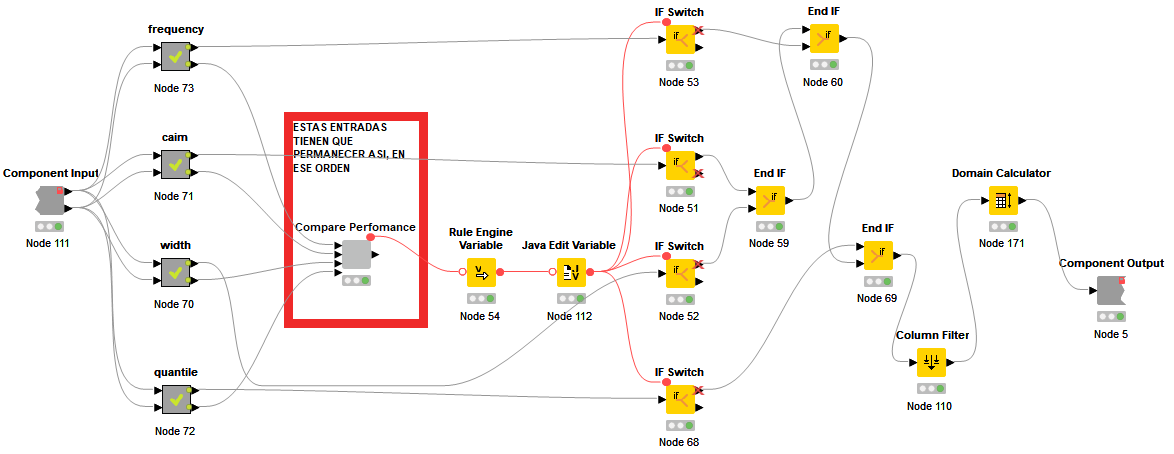
\includegraphics[width=\textwidth]{figuras/anexos/discretizer}
	\caption{Flujo KNIME del componente \textit{Discretizer}}
	\label{anex:discretizer}
\end{figure}


\chapter{Ejemplo de discretización \textit{Equal-Frequency} para el modelo ID3} \label{aped:9}
%\addcontentsline{toc}{section}{Anexo IX: Ejemplo de discretización\textit{Equal-Frequency} para el modelo ID3}

\begin{figure}[H]
	\centering
	\includegraphics[width=\textwidth]{"figuras/anexos/ejemplo discretizacion freq id3"}
	\caption{Flujo KNIME para la discretización\textit{ Equal-Frequency} en el modelo ID3}
	\label{anex:ejemplo-discretizacion-freq-id3}
\end{figure}

\chapter{Flujo KNIME del componente\textit{ MV Imputation}} \label{aped:10}
%\addcontentsline{toc}{section}{Anexo X: Flujo KNIME del componente \textit{MV Imputation}} 

\begin{figure}[H]
	\centering
	\includegraphics[width=\textwidth]{"figuras/anexos/MV Imputation"}
	\caption{Flujo KNIME del componente \textit{MV Imputation}}
	\label{anex:mv-imputation}
\end{figure}

\chapter{Flujo KNIME del componente \textit{Normalizer}} \label{aped:11}
%\addcontentsline{toc}{section}{Anexo XI: Flujo KNIME del componente \textit{Normalizer}}
	
\begin{figure}[H]
	\centering
	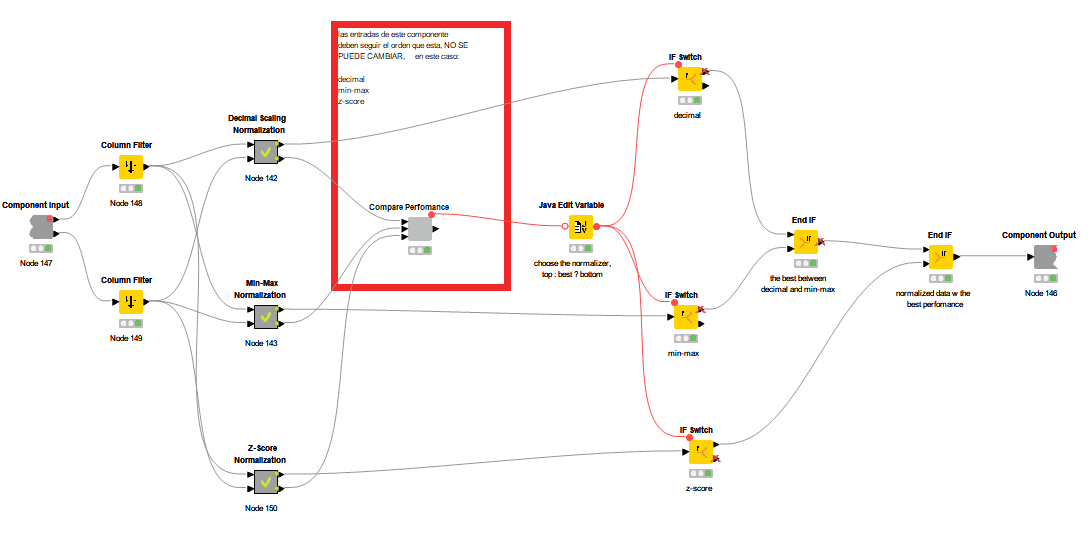
\includegraphics[width=\textwidth]{figuras/anexos/normalizer}
	\caption{Flujo KNIME del componente \textit{Normalizer}}
	\label{anex:normalizer}
\end{figure}
	

\chapter{Ejemplo de normalización \textit{Decimal Scaling} para el modelo PNN}\label{aped:12}
%\addcontentsline{toc}{section}{Anexo XII: Ejemplo de normalización \textit{Decimal Scaling} para el modelo PNN} \label{aped:12}

\begin{figure}[H]
	\centering
	\includegraphics[width=\textwidth]{"figuras/anexos/ejemplo normalizacion pnn decimal scaling"}
	\caption{Flujo KNIME para la normalización \textit{Decimal Scaling} en el modelo PNN}
	\label{anex:ejemplo-normalizacion-pnn-decimal-scaling}
\end{figure}

\chapter{Componente \textit{AutoML Clasificación}} \label{aped:13}
%\addcontentsline{toc}{section}{Anexo XII: Componente \textit{AutoML Clasificación}} 

\begin{figure}[H]
	\centering
	\includegraphics[width=\textwidth]{"figuras/anexos/componente integrado"}
	\caption{Flujo KNIME del componente \textit{AutoML Clasificación}}
	\label{anex:componente-integrado}
\end{figure}

\chapter{Ejemplo de integración de componentes al modelo PNN} \label{aped:14}
%\addcontentsline{toc}{section}{Anexo XIV: Ejemplo de integración de componentes al modelo PNN} 

\begin{figure}[H]
	\centering
	\includegraphics[width=\textwidth]{"figuras/anexos/ejemplo integracion componentes pnn"}
	\caption{Flujo KNIME de la integración de los componentes al modelo PNN}
	\label{fig:ejemplo-integracion-componentes-pnn}
\end{figure}


\chapter{Métodos de normalización elegidos acorde al \textit{dataset} y modelo} \label{aped:15-normalizacion}
En la tabla \ref{tabla-normalizacion} se muestra como tras la ejecución y evaluación de los normalizadores y de ejecutar el algoritmo de Aprendizaje Automático en cuestión, se escoge de forma automatizada el que mejor desempeño obtiene. Estos resultados destacan la influencia significativa del método de normalización en el rendimiento de los modelos de ML y cómo esta elección puede depender tanto del conjunto de datos específico como del algoritmo utilizado. 

\begin{table}
	\centering
	\caption{Métodos de normalización utilizados en cada \textit{dataset} para cada modelo}
	\label{tabla-normalizacion}
	\begin{tabular}{|l|l|l|} 
		\hline
		\textbf{\textit{Dataset}}                 & \textbf{Modelo} & \textbf{Método auto-seleccionado}  \\ 
		\hline
		\multirow{2}{*}{\textsc{dry bean}}        & PNN             & Z-score                            \\ 
		\cline{2-3}
		& SVM             & Z-score                            \\ 
		\hline
		\multirow{2}{*}{\textsc{human resources}} & PNN             & Decimal Scaling                    \\ 
		\cline{2-3}
		& SVM             & Z-score                            \\ 
		\hline
		\multirow{2}{*}{\begin{tabular}[c]{@{}l@{}}\textsc{water quality}\\\textsc{and potability}\end{tabular}} & PNN             & Z-score                            \\ 
		\cline{2-3}
		& SVM             & Decimal Scaling                    \\
		\hline
	\end{tabular}
\end{table}

\chapter{Métodos de discretización elegidos acorde al \textit{dataset} y modelo} \label{aped:16-discretizacion}
En la tabla \ref{tabla-discretizacion} se muestra como tras la ejecución y evaluación de los discretizadores y de ejecutar el algoritmo de Aprendizaje Automático en cuestión, se escoge de forma automatizada el que mejor desempeño obtiene. Estos resultados subrayan la variabilidad en la elección del método de discretización en función tanto del conjunto de datos como del modelo de aprendizaje automático. 

\begin{table}
	\centering
	\caption{ Métodos de discretización utilizados en cada \textit{dataset} para cada modelo}
	\label{tabla-discretizacion}
	\begin{tabular}{|l|l|l|} 
		\hline
		\textit{\textbf{Dataset}}                                                                                   & \textbf{Modelo} & \textbf{Método auto-seleccionado}  \\ 
		\hline
		\multirow{2}{*}{\textsc{cancer data}}                                                              & ID3    & CAIM                      \\ 
		\cline{2-3}
		& C4.5   & CAIM                      \\ 
		\hline
		\multirow{2}{*}{\begin{tabular}[c]{@{}l@{}}\textsc{academic} \\ \textsc{success} \end{tabular}}               & ID3    & Equal Frequency           \\ 
		\cline{2-3}
		& C4.5   &  Equal Frequency           \\ 
		\hline
		\multirow{2}{*}{\textsc{census income}}                                                            & ID3    & CAIM                      \\ 
		\cline{2-3}
		& C4.5   & Equal Width               \\ 
		\hline
		\multirow{2}{*}{\begin{tabular}[c]{@{}l@{}}\textsc{airline passenger} \\ \textsc{satisfaction} \end{tabular}} & ID3    & Equal Width               \\ 
		\cline{2-3}
		& C4.5   &  Equal Frequency           \\
		\hline
	\end{tabular}
\end{table}

\chapter{Métodos de imputación de valores faltantes elegidos acorde al \textit{dataset} y modelo} \label{aped:17-mv-imp}
En la tabla \ref{tabla-mv-imp-comparativa} se muestra como tras la ejecución y evaluación de los métodos de imputación de valores perdidos y de ejecutar el algoritmo de Aprendizaje Automático en cuestión, se escoge de forma automatizada el que mejor desempeño obtiene.
Estos resultados revelan la variabilidad en la elección de métodos de imputación de datos faltantes en función tanto del conjunto de datos específico como del modelo de aprendizaje automático. 


\begin{table}
	\centering
	\caption{Métodos de imputación de valores faltantes utilizados en cada \textit{dataset} para cada modelo}
	\label{tabla-mv-imp-comparativa}
	\begin{tabular}{|l|l|l|} 
		\hline
		\textbf{\textit{Dataset}}                                                                          & \textbf{Modelo} & \textbf{Método auto-seleccionado}  \\ 
		\hline
		\multirow{4}{*}{\textsc{human resources}}                                                          & ID3             & kMI                                \\ 
		\cline{2-3}
		& C4.5            & kMI                                \\ 
		\cline{2-3}
		& CART            & kMI                                \\ 
		\cline{2-3}
		& PNN             & kMI                                \\ 
		\hline
		\multirow{3}{*}{\textsc{census income}}                                                            & ID3             & kNNI                               \\ 
		\cline{2-3}
		& C4.5            & kNNI                               \\ 
		\cline{2-3}
		& CART            & kNNI                               \\ 
		\hline
		\multirow{6}{*}{\begin{tabular}[c]{@{}l@{}}\textsc{airline passenger} \\ \textsc{satisfaction} \end{tabular}} & ID3             & kMI                                \\ 
		\cline{2-3}
		& C4.5            & kMI                                \\ 
		\cline{2-3}
		& CART            & kNNI                               \\ 
		\cline{2-3}
		& PNN             & kNNI                               \\ 
		\cline{2-3}
		& RPROP           & kMI                                \\ 
		\cline{2-3}
		& SVM             & kNNI                               \\ 
		\hline
		\multirow{6}{*}{\begin{tabular}[c]{@{}l@{}} \textsc{water quality}\\\textsc{ and potability} \end{tabular}}    & ID3             & kMI                                \\ 
		\cline{2-3}
		& C4.5            & kMI                                \\ 
		\cline{2-3}
		& CART            & kNNI                               \\ 
		\cline{2-3}
		& PNN             & kMI                                \\ 
		\cline{2-3}
		& RPROP           & kMI                            \\ 
		\cline{2-3}
		& SVM             & kNNI                               \\
		\hline
	\end{tabular}
\end{table}

